\chapter{REAL-TIME PARTICLE SYSTEMS LIBRARY}\label{RTPSchapter}

% Introduction
\section{Introduction}
The Real-Time Particle Systems (RTPS) library was designed and developed by Ian Johnson\cite{ianPaper}. RTPS is capable to simulate various particle systems including Smooth Particle Hydrodynamics (SPH) and Flocking (Boids) systems. In collaboration with Ian Johnson, a \texttt{FLOCK} system was created.

This chapter will introduce the RTPS framework. The description of the RTPS library will follow the structure of the RTPS implementation. At the end of the chapter a detailed description of the extended implementation developed for the \texttt{FLOCK} system is going to be given. 

% RTPS diagram
\begin{figure}[htbp]
\begin{center}
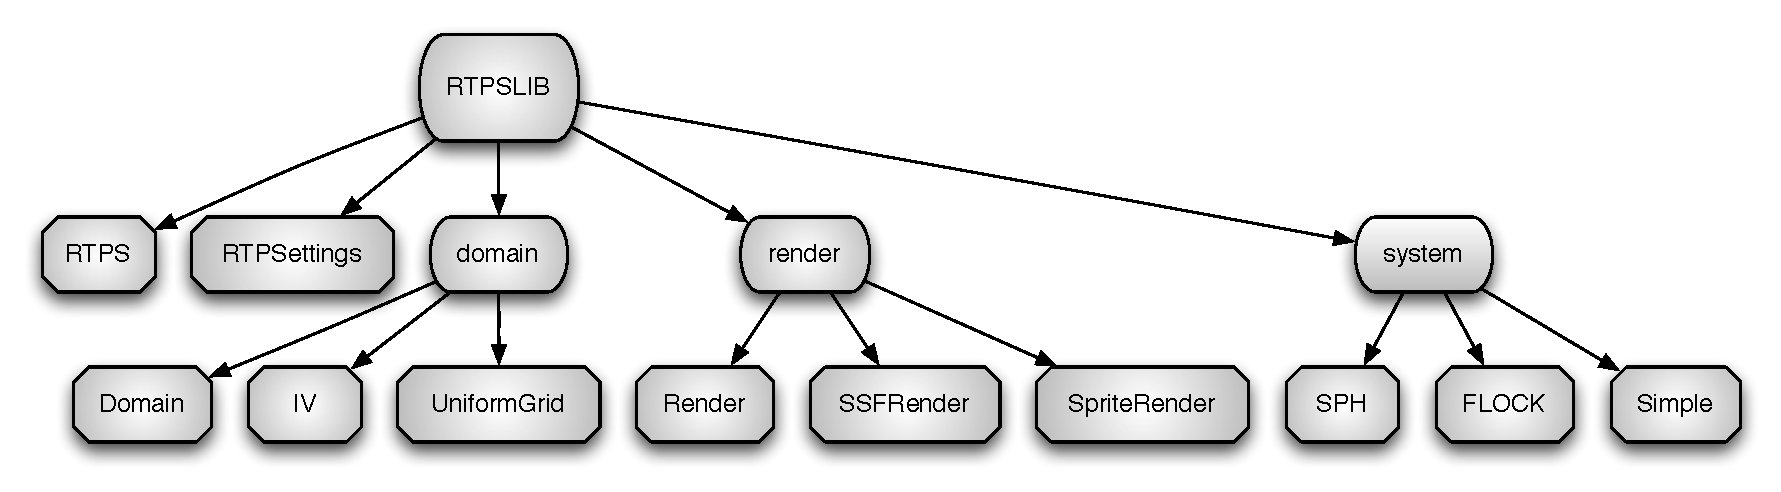
\includegraphics[scale=0.30]{figures/RTPSdiagram.pdf}
\caption{RTPS dependency diagram}
\label{RTPSdiagram}
\end{center}
\end{figure}

% RTPS
\section{RTPS}\label{rtpssection}
\texttt{RTPS.h} is the head class of the RTPS library. An \texttt{RTPS} object is a particle system, this system may be initialized with given a set of settings. The settings are going to be discussed in Section~\ref{rtpsettings}. 

As can be seen in Figure~\ref{RTPSdiagram}, \texttt{RTPS} its included in various classes which are going to be discussed later in this chapter. Only two methods are defined in this class: \texttt{update()} and \texttt{render()}. \texttt{update()} will compute the next positions of the particles, while \texttt{render()} is in charge of rendering the particles. These methods are implemented individually by each of the systems available in the RTPS library. The following code represents the definition of the \texttt{RTPS} constructor used when creating the \texttt{FLOCK} system.

%\texttt{RTPS} has various instance variables: a \texttt{CL} object which is used to manage the \textit{OpenCL} functionality,  an \texttt{RTPSettings} object to manage the settings of the system and a \texttt{System} object which stores the type of particle system that has been created. 
% RTPS constructor

\begin{cppcode}{0}
RTPS::RTPS(RTPSettings *s, CL* _cli) 
{
	cli = _cli;
 	cl_managed = false;
	settings = s;
	Init();
}
\end{cppcode}

The \texttt{Init()} method that is called inside the constructor would creates the respective particle system, i.e. \texttt{SPH} or \texttt{FLOCK}, depending on the settings.

% RTPSettings
\section{RTPS Settings}\label{rtpsettings}
\texttt{RTPSettings} is the class that stores all the settings of the particle systems. This class defines the set of systems available in RTPS. Depending on the systems the settings are defined. The three systems currently available are: SPH, FLOCK and Simple. The constructor used to create the RTPS  settings is presented bellow. \texttt{Systype} is an enumeration that has the name of the systems stated above.

%The location of this class is at \texttt{rtpslib/RTPSettings.h}. It has the following instance variables defined: the maximum number of particles, the time step, and a \texttt{Domain} object. Also, there is an enumeration variable \texttt{SysType} that defines the names of the three available particle systems. Some of the rendering settings are set and get in this class. Here is the \texttt{RTPSettings} constructor that we use for the \texttt{FLOCK} system.

% RTPSettings constructor
\begin{cppcode}{0}
RTPSettings::RTPSettings(SysType system, int max_particles, float dt, Domain* grid)
{
	changed = false;
	this->system = system;
	this->max_particles = nlpo2(max_particles);
	this->dt = dt;
	this->grid = grid;
}
\end{cppcode}

%The parameters for this constructor are the type of system, the maximum number of particles, the time step and the grid domain. 

As an OpenCL requirement the maximum number of particles has to be a power of two. That is why the variable \texttt{max\_particles} is processed through the function \texttt{nlpo2}, which takes care of that.

% Domain
\section{Domain}
The \texttt{Domain} class defines the grid in which the simulation is being computed. This class also stores all the different grid parameters that are needed through out the computation process. The \texttt{IV} class is defined in the same folder than the \texttt{Domain} class. The \texttt{IV} class defines and implements the methods that initialize the positions of the particles. Various geometric shapes are available: rectangles, spheres, and discs. The \texttt{UniformGrid} class is also defined in the same folder than the \texttt{Domain} class. \texttt{UniformGrid} class is used for the nearest neighbor search.

% Render
\section{Render}
Most of the code developed to do the render for the RTPS library was developed by Andrew Young\footnote{http://andrewfsu.blogspot.com/}. There are few classes that are in charge of the rendering process. Those classes are \texttt{Render}, \texttt{SpriteRender}, \texttt{SSFRender}. The \texttt{Render} renders the particles as points. The \texttt{SpriteRender} class uses images that are mapped to spheres. A special shader was developed for the use of sprites for boids rendering. This special shader let us render a 2D image with transparent background as a boid.

% System
\section{System}
Each of the particle systems in the RTPS library inherits the \texttt{System} class which contains virtual functions that are shared by the systems. These functions are related to the rendering,  the domain, and other shared classes. There are three systems that extends the \texttt{System} class. Those systems are: \texttt{SPH}, \texttt{FLOCK}, and \texttt{Simple}. The \texttt{SPH} system is going to be briefly discussed in Section~\ref{sphsection}. The \texttt{FLOCK} system would be described in detail in Section~\ref{flocksection}. Finally, the \texttt{Simple} system was created for testing and debugging the \texttt{SPH} system.

% Common
\section{Common}\label{commonsection}
Inside the \texttt{rtpslib/system/common} folder are the classes that are shared by the systems. In this folder there is the implementation of the nearest neighbor search and the hose which is used to insert particles to the systems. Hoses are very useful for doing different kinds of demonstrations. 

The next section explains how the nearest neighbor search is done. 

\subsection{Nearest Neighbor Search}
The approach taken to do the implemented nearest neighbor search is divided in two phases: \textit{preparation} and \textit{lookup}. The step to do the preparation are the following:

\begin{enumerate}
\item{\textbf{Hash}: creates a hash value by overlaying a uniform grid at the system's domain, and calculating a index value from the 3D cell index}
\item{\textbf{Sort}: sorts the hash array by the hash values, an array with the initial indices of the particles is also sorted according the hash values}
\item{\textbf{Permute}:  permutes the arrays of positions, velocities, veleval and color according to the sorted index array}
\item{\textbf{Cell indices}: updates two arrays: \texttt{cell\_indices\_start} and \texttt{cell\_indices\_end} which keep track of which cell are populated with particles, \texttt{cell\_indices\_start} stores the index of the first particle in each cell, when there is no particle an index of $-1$ is assigned while \texttt{cell\_indices\_end} stores the index of the last particle in that cell}
\end{enumerate}

After the preparation is done arrays are ready to be access it, this meaning that are ready for the neighbor searching. The access of  the arrays is made during the lookup phase of the nearest neighbor search. This phase consist of calling the following three functions:

\begin{enumerate}
\item{\textbf{IterateParticleInNearbyCells}: loops over the 26 cells surrounding the cell of the particle in question, this function calls \texttt{IterateParticlesInCells} for each cell }
\item{\textbf{IterateParticlesInCells}: loops over the particles from the start index to the end index of that cell and calls \texttt{ForNeighbor} for each particle}
\item{\textbf{ForNeighbor}: access the particle in question and the neighboring particle}
\end{enumerate}

Having the particle information and the neighbor particle information, then the respective computations are done between them. Each of the rules of flocking implemented here uses the nearest neighbor search, therefore we do the lookup for each rule independently.

% SPH
\section{SPH}\label{sphsection}
The \texttt{SPH} system is the main system of the RTPS library. It was developed and it is currently maintained by Ian Johnson\footnote{http://enja.org/}\cite{ianPaper}. This system uses the SPH formulation to compute the different forces between particles.

The difference only between the \texttt{FLOCK} system and the \texttt{SPH} is the calculation of the forces. The algorithm followed is very very similar. The SPH formulation is used to compute forces while the boids only need to compute their steering behaviors. At the end both systems have a new velocity that is used to update the positions of the particles.

For a more detailed information about the \texttt{SPH} system implemented in the RTPS library, please refer to Ian Johnson Master Thesis\cite{ianThesis}.

% FLOCK
\section{FLOCK}\label{flocksection}
The \texttt{FLOCK} system is the system of our concern. As mentioned in the previous Section, the \texttt{SPH} system was used as a guide to create the \texttt{FLOCK} system. Both of these systems are extends the \texttt{System} class. The main class of the \texttt{FLOCK} system is also called \texttt{FLOCK}. Also, a class for the settings of the \texttt{FLOCK} system was developed. This class was called \texttt{FLOCKSettings}. The three basic steering behaviors of flocking were implemented. Figure~\ref{flockdiagram} shows the hierarchy of the \texttt{FLOCK} system. In the first layer are some of the classes that are included in the \texttt{FLOCK.h} class and not mentioned in Figure~\ref{RTPSdiagram}. These classes are going to be discussed in this Section with an exemption of the shared classes which are \texttt{Hash}, \texttt{BitonicSort}, \texttt{Permute}, \texttt{CellIndices} and \texttt{Hose}. A brief description brief description of these classes is at Section~\ref{commonsection}.

% FLOCK diagram
\begin{figure}[htbp]
\begin{center}
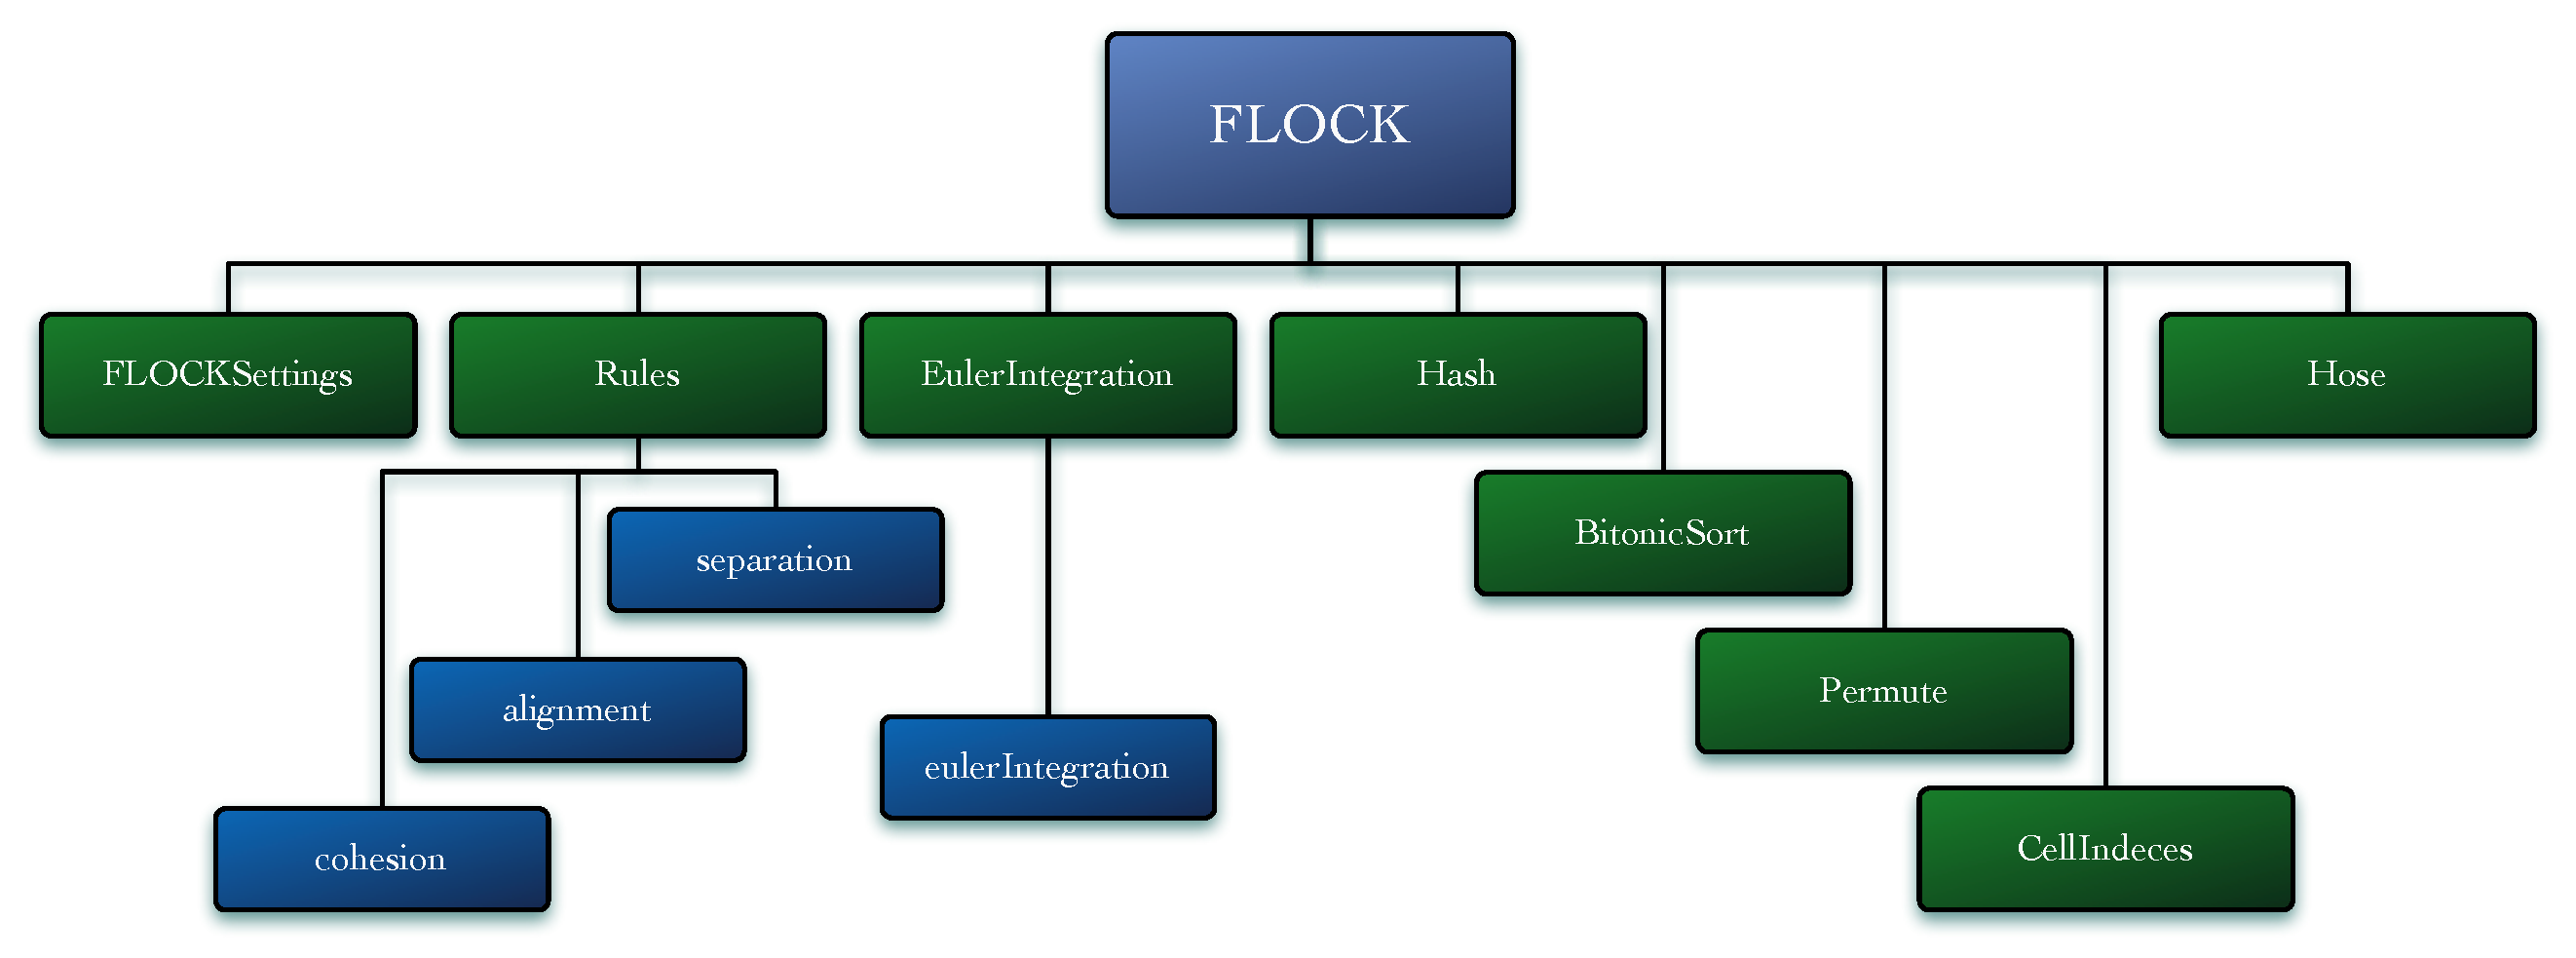
\includegraphics[scale=0.3]{figures/FLOCKdiagram.pdf}
\caption{FLOCK hierarchy diagram}
\label{flockdiagram}
\end{center}
\end{figure}


The remaining of this Section will talk about the implementation of the \texttt{FLOCK} system.

% FLOCK class
\subsection{FLOCK class}
As mentioned before the \texttt{FLOCK} class is the main class of our system. The header file defines the prototypes of the functions that are used to insert particles into our system. Also, all the vectors and buffers used to store the information of of the particles in the CPU and GPU are declared in this class. The following code shows some of the main step in the constructor of our class.

\begin{cppcode}{0}
FLOCK::FLOCK(RTPS *psfr, int n)
 {
 	//store the particle system framework
 	ps = psfr;
	settings = ps->settings;
	grid = settings->grid;
	max_num = n;
	
	// initial number of particles
	num = 0;
 	
	...
 
 	// calculate and update the parameters
	calculate();
	updateFLOCKP();

	...

	//set up the grid
	setupDomain();
	
	//setup the sorted and unsorted arrays
	prepareSorted();
 	 
	 ...
		
	// create the renderer object depending on the render type		
	setRenderer(); 
}
\end{cppcode}

At the beginning some of the instance variables of \texttt{FLOCK} are set to the respectives values obtained from the arguments. 

Then, the initial settings of the system are calculated and updated. The settings of \texttt{FLOCK} are stored in a struct called \texttt{FLOCKParameters}. When doing executing \texttt{calculate()}, the parameters are set to the default values. Then the \texttt{updateFLOCKP()} is called and the parameters are updated, this is made in case that the some of the parameters were set by the user, then the struct would show the updated values. 

The next important step is to set the domain. During the setup of the domain the grid parameters are initalized.

Then, the function \texttt{prepareSorted()} is called. What \texttt{prepareSorted()} does is to initialize the different vectors and buffers that were created i.e \texttt{velocities}, \texttt{flockmates}, etc. This function also creates the VBOs. VBOs stands for Vertex Buffer Objects and what this buffer objects are used to store vertex data that its aim to be used for rendering purposes\footnote{http://www.songho.ca/opengl/gl\_vbo.html}. Then, the positions and color vectors are copied to the respective VBOs. If using the GPU the different \texttt{Buffer} objects are initialized with their respective CPU arrays. The \texttt{FLOCK} parameters are also copied to the GPU. 

Finally, the \texttt{setRenderer()} function is called, and it creates the \texttt{renderer} object depending on which render type was set in the \texttt{RTPSettings}.


\subsubsection{Particles insertion}
The system has being created now the question is \textit{how do the particles are inserted into the system?} There are a few functions defined in the \texttt{FLOCK} that do that task. These functions are \texttt{addBox} , \texttt{addBall}, and \texttt{addHose}. First, these function initialize the positions of the particles using the functions defined in \texttt{IV.h} class which is the Initial Values class, then the positions of the particles are send it to the GPU or CPU to be rendered. 

\subsubsection{Update}
As mentioned in Section~\ref{rtpssection} each of the systems would implement the methods \texttt{update()} and \texttt{render()}, respectively. In \texttt{FLOCK} the \texttt{update()} function updates the positions of the boids at each time step. If using the CPU, the \texttt{updateCPU()} function is called. \texttt{updateCPU()}  only calls the function \texttt{cpuRules()} which computes the rules sequentially in the CPU. The CPU code was developed for testing and debugging purposes only. On the other hand, if using the GPU to do the calculations, the \texttt{updateGPU()} function is called. \texttt{updateGPU()} calls the OpenCL kernels that do the nearest neighbor search and then compute the flocking rules. These kernels are going to be described in more detail in Section~\ref{rulesclass}.


% FLOCKSettings class
\subsection{FLOCKSettings class}
In order to run a simulation the settings of the system need to be set. The flocking specific settings are defined in the class called \texttt{FLOCKSettings}. The \texttt{FLOCKParameters} struct is defined in this same class. 

The parameters of the \texttt{FLOCKParameters} struct include: the simulation scale, the searching radius, the maximum speed of the boids and the weights of each of the steering behaviors. In the implementation file of the \texttt{FLOCKSettings} class are the respective implementations of the functions \texttt{calculate()} and \texttt{updateFLOCKP()}.

% Rules class
\subsection{Rules class}\label{rulesclass}
The \texttt{Rules} class defines the different steering behaviors that were implemented to simulate the flocking behavior. The steering behaviors or \textit{rules} are implemented in both CPU and GPU code. Each of the rules implemented for the GPU execution is defined in an independent kernel. The following code is the \texttt{Rules.h} file which defines the \texttt{Rules} class.

\begin{cppcode}{0}
#ifndef RTPS_RULES_H_INCLUDED
#define RTPS_RULES_H_INCLUDED

#include <CLL.h>
 #include <Buffer.h>

namespace rtps
 {
	class Rules
	{
		public:
			// constructors
			Rules() { cli = NULL; timer = NULL; };
			Rules(std::string path, CL* cli, EB::Timer* timer);
			
			// execution of kernels
			void executeFlockmates( /* arguments */ );
			void executeSeparation( /* arguments */ );
			void executeAlignment( /* arguments */ );
			void executeCohesion( /* arguments */ );
			
		private:
			// OpenCL
			CL* cli;
			
			// kernels
			Kernel k_flockmates;
			Kernel k_rule_separation;
			Kernel k_rule_alignment;
			Kernel k_rule_cohesion;
			
			// timer
			EB::Timer* timer;
	};
}
#endif
\end{cppcode}

The implementation of each of the functions that executes the kernels is in \texttt{Rules.cpp}. First, the kernels are initialized in the constructor of the \texttt{Rules} class, then in the implementation of the functions that executes the kernels, the arguments of the kernels are set. In this file \texttt{Rules.cpp} is where the \texttt{cpuRules()} function is implemented. Part of the \texttt{Rules.cpp} file is shown next.

\begin{cppcode}{0}
#include<FLOCK.h>
#include<math.h>

namespace rtps
{
	// Rules constructor
	Rules::Rules(std::string wpath, CL* cli_, EB::Timer* timer_)
	{
		...
		try
		{
			path = wpath + "/flockmates.cl";
			k_flockmates = Kernel(cli, path, "flockmates");
		}
		....
	}

	// flockmates
	void Rules::executeFlockmates( /* arguments */ )
	{
		// set the arguments for the kernel
		int iarg = 0;
		k_flockmates.setArg(iarg++, pos_s.getDevicePtr());
		k_flockmates.setArg(iarg++, neigh_s.getDevicePtr());
		...
	}
	...
	
	void FLOCK::cpuRules()
	{
		...
	}
}
\end{cppcode}

The implementation of the kernels was done in a separate folder. This would help us to better distinguish between the C++ and the OpenCL files. The kernels defined in \texttt{Rules} are called \texttt{flockmates}, \texttt{rule\_separation}, \texttt{rule\_alignment}, and \texttt{rule\_cohesion}. %, and \texttt{rule\_leaderfollowing}.

\texttt{\textbf{flockmates}} looks for the neighbors and determines which ones are within the searching radius, and count them. Also, it counts how many neighbors are within the minimum separation distance of each boid. At the end, the vector \texttt{flockmates} which was allocated in the GPU is updated with the values obtained.

\texttt{\textbf{rule\_separation}} is computed using the neighbors that are within the minimum separation distance\footnote{for more details on how the rule is computed see the formulation of Separation in Section~\ref{separationsection}}. The behavior is accumulated in a vector. After the neighbors within the minimum distance are processed, the behavior vector is averaged over the number of flockmates found within the minimum separation distance, then the vector is normalized. Finally, the value of the vector \texttt{separation} are copied to the vector allocated in the GPU.

\texttt{\textbf{rule\_alignment}} determines which neighbors are within a prescribed radius, the velocities of those neighbors are accumulated. Then, the average is taken using the number of flockmates following by a subtraction of the average velocity and the boids velocity. At the end the vector obtained is used to update the respective vector in the GPU. 

\texttt{\textbf{rule\_cohesion}} is analogous to the alignment rule, the only difference is that positions are used instead of velocities.

%\texttt{\textbf{rule\_leaderfollowing}} \textcolor{red}{*** TODO: still need to develop the leader behavior, then I would write the description of this kernel ***}

This would finish the description of the \texttt{Rules} class. The next step is to integrate over time to get the new position of the boid.

% Euler Integration class
\subsection{EulerIntegration class}
A discussion on how to get the different steering behaviors vectors have been done. Now a brief explanation on how to combine the behaviors in order to get one single vector to update the positions is going to be given. A class called \texttt{EulerIntegration} have been developed in order to do that. The code of the {EulerIntegration.h} class is stated bellow.

\begin{cppcode}{0}
#ifndef RTPS_EULER_INTEGRATION_H_
#define RTPS_EULER_INTEGRATION_H_

#include <CLL.h>
#include <Buffer.h>

namespace rtps
{
	class EulerIntegration
	{
		public:
			EulerIntegration() { cli = NULL; timer = NULL; };
	 		EulerIntegration(std::string path, CL* cli, EB::Timer* timer);
			void execute( /* arguments */ );

		private:
			CL* cli;
			Kernel k_euler_integration;
			EB::Timer* timer;
	};
}
#endif
\end{cppcode}

The \texttt{EulerIntegration} class structure is similar to the \texttt{Rules} class structure. That means that the \texttt{EulerIntegration.cpp} would initialize the kernel and implement the \texttt{execute} function which sets the arguments of the kernels and executes it. It also has the \texttt{cpuEulerIntegration()} function implementation. The name of the kernel developed for the integration in the GPU is \texttt{euler\_integration}, it is also located in the same folder along with the rules kernels.

\texttt{\textbf{euler\_integration}} starts by getting the respective steering vectors from the GPU, and also getting the weights of each of the rules. The weights are gotten from the flocking parameters object. Then, the acceleration vectors for each of the rules are computed and combined to get the final acceleration vector.

\begin{cppcode}{0}
// RULE 1. SEPARATION
acc_sep = separation * w_sep;
   
// RULE 2. ALIGNMENT
acc_aln = alignment * w_aln;

// RULE 3. COHESION
acc_coh = cohesion * w_coh;

// GLOBAL ACCELERATION
acc = vi + acc_sep + acc_aln + acc_coh;
\end{cppcode}

After obtaining the global acceleration vector, this vector is constrained to the maximum speed. 

An optional circular velocity field that modifies the acceleration can be added to the boids acceleration. The constant that weights how strong this velocity field is going to be is stored in the flocking parameters.

\begin{cppcode}{0}
// OPTIONAL CIRCULAR VELOCITY FIELD
float4 v = (float4)(-3*pi.z, 0.f , pi.x, 0.f);
v *= flockp->circular_vel_const;

// ADD THE ACCELERATION AND OPTIONAL CIRCULAR VELOCITY TO THE VELOCITY
vi = v + acc;
vi.w = 0.f;

// INTEGRATION
pi += dt*vi; 
\end{cppcode}

Finally, the integration over time time is done to get the next position of each boid. This is followed by making sure that boids stay inside the domain by applying periodic boundary conditions to them. 

This description cover what happens at each step of the simulation for each boid. This algorithm would repeat in real-time until the user quits the program.

